\documentclass[letterpaper,12pt]{article}
\usepackage[utf8]{inputenc}
\makeatletter
\renewcommand{\@seccntformat}[1]{%
  \ifcsname specialformat#1\endcsname
    \csname specialformat#1\endcsname
  \else
    \csname the#1\endcsname\quad % default
  \fi
}
\makeatother
\newcommand{\specialformatsection}{}
\renewcommand{\thesubsection}{\arabic{subsection}}
\usepackage[T1]{fontenc}
\usepackage{charter}
\usepackage{geometry}
\usepackage{amsmath}
\usepackage{float}
\usepackage{graphicx}
\usepackage{subcaption}
\usepackage{amssymb}
\usepackage{adjustbox}
\usepackage{wrapfig} %%imagen envuelta por un texto
\usepackage{xcolor}
\usepackage{fancyhdr}
\usepackage{tabularx} %%TABLAS OH YEAH

\title {\textbf{Análisis de la Demanda}}
\author{Lara Xocuis Martha Denisse}
\date{24 de noviembre de 2023}
\geometry{top=2cm, bottom=2cm, left=2cm, right= 2cm} %%margen
\graphicspath{{images/}}
\parindent=0pt
\begin{document}
\maketitle
\newpage
%%%%%%%%%%%%%%%%%%%%%%%%%%%%%%%%%%%%%%%%%%%%%%%%%%%%%%%%%%%%%%%%%%%%%%%%%%%%
\begin{sloppypar}
\section{Servicios que tienen mayor demanda}
\begin{figure}[H]
  \centering 
  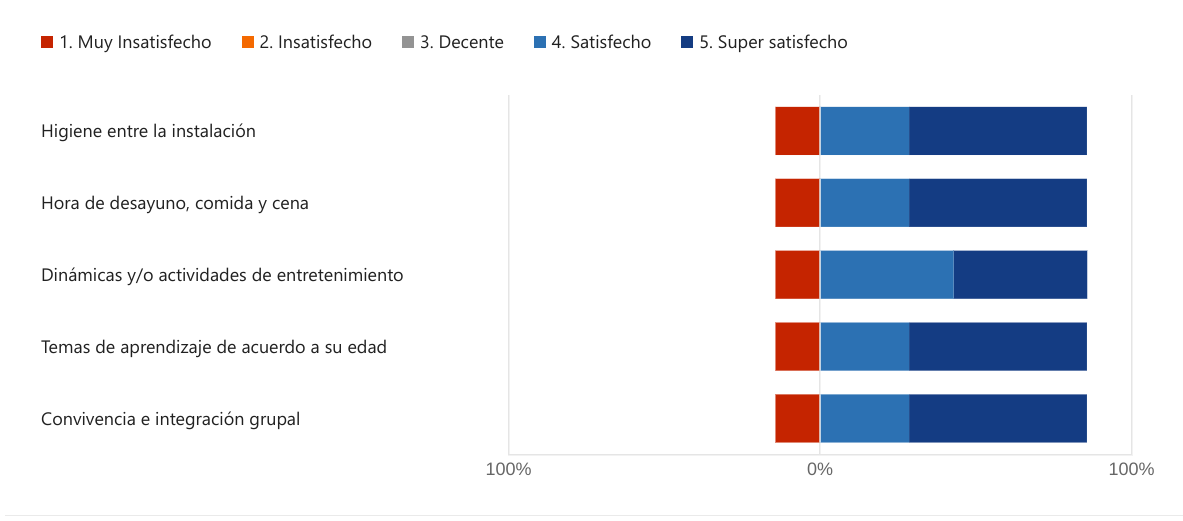
\includegraphics[width=0.9\textwidth]{demanda1.png}
\end{figure}

\begin{figure}[H]
  \centering 
  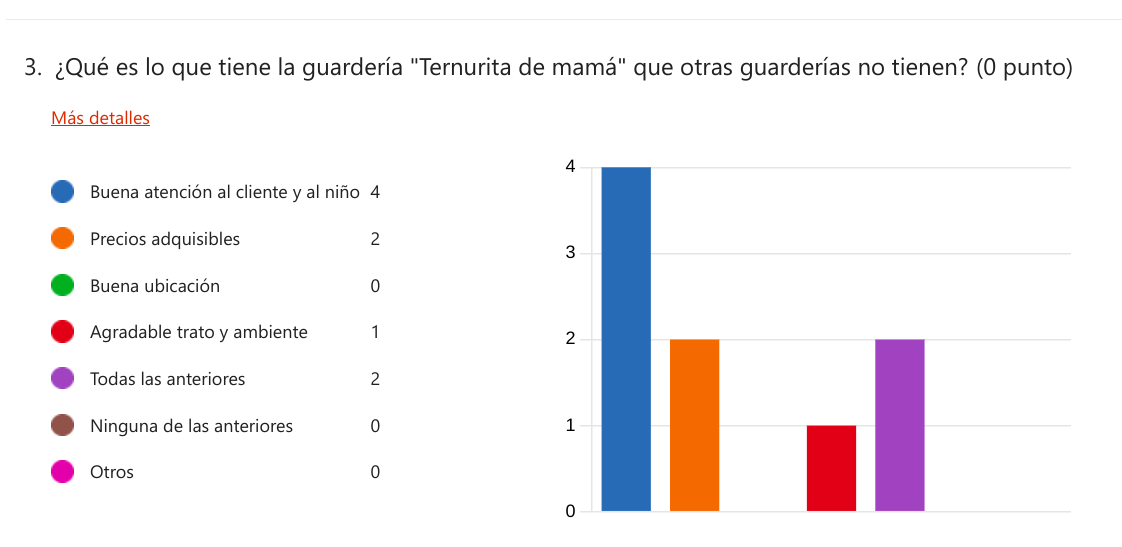
\includegraphics[width=0.9\textwidth]{demanda2.png}
\end{figure}
Según las gráficas y adaptando a las respuestas que se pudieron recolectar de las encuestas anteriores, se observa que la atención al cliente es la característica más destacada. En términos generales, los servicios dirigidos a los niños, como alimentación, actividades recreativas y aspectos educativos, son los más demandados por los padres. Esto sugiere que existe una alta prioridad en la satisfacción y el bienestar de los niños, con un énfasis particular en las interacciones y servicios que directamente impactan en su desarrollo, educación y calidad de vida.
\section{Estrategias}
\subsubsection{Sostener la demanda actual}
Para sostener la demanda de servicios centrados en la atención al cliente y en las necesidades de los niños, se pueden implementar diversas estrategias que fortalezcan la oferta y generen una conexión duradera con los clientes.
\begin{itemize}
  \item Priorizar atención al cliente: Mantenerse y tener un servicio al cliente de forma excepcional, seguir con las expectativas de los padres. También es importante implementar sistemas de retroalimentación sugerencias sugerencias de los padres. 
  \item Temas educacionales para los niños: Implementar elementos con buenas bases para el aprendizaje de los niños, adaptar cada programa para cada niño.  Mantenerse al tanto de las últimas tendencias educativas y ajustar continuamente los programas garantiza que se ofrezcan servicios de calidad y relevancia.
  \item Seguridad del niño: Implementar medidas sólidas de seguridad y comunicarlas de manera transparente a los padres genera confianza. Establecer protocolos claros para situaciones de emergencia demuestra un compromiso serio con la seguridad.
  \item Actividades recreativas: Organizar eventos regulares y actividades grupales promueve la convivencia y fortalece los lazos entre la comunidad. Ofrecer descuentos o incentivos para la participación en estas actividades no solo mejora la satisfacción del cliente, sino que también puede generar lealtad a largo plazo.
\end{itemize}

\subsubsection{Mejorar la demanda de productos / servicios que no se vendan igual}
\begin{itemize}
  \item Creatividad: Ofrecer una amplia variedad de dinámicas y actividades de entretenimiento para los niños, que abarque desde juegos educativos hasta actividades artísticas y deportivas para mantener a los niños comprometidos y emocionados.
  \item Entorno:  Asegurarse de que las instalaciones cumplan con los estándares de seguridad, tener un ambiente acogedor, colorido, organizado y llamativo para mantener un ambiente positivo entre los niños.
  \item Ubicación: Asegurarse de que la guardería sea fácilmente accesible y que los padres se sientan seguros al dejar a sus hijos. Identificar y destacar servicios complementarios en la zona (doctores, supermercados o áreas de juegos).
  \item Personal: Equipo amable, carismático, profesional, y bien capacitado para crear un entorno seguro y acogedor para los niños y los padres.
\end{itemize}
\newpage
\section{Conclusión}
Para mejorar la demanda de servicios en una guardería es importante
enfocarse en las expectativas de los padres. La guardería debe destacarse sobre los servicios que provee. Entre muchas pautas ya mencionadas para manter y mejorar la demanda de productos, implica tener una estrategia para dicha calidad de servicio y fomentar la lealtad del cliente. 
\vspace{0.3cm}\\ 
Es realmente relevante implementar estas estrategias para un cambio de perspectiva y adaptabilidad dentro de la guardería, ayudaría muchísimo a la satisfacción de los padres y niños para aumentar dicha demanda.

\section{Aprendizaje}
Es importante comprender y saber las necesidades de los padres, y es que es su principal cliente, se debe de dar la preferencia a este mismo para saber cómo y dónde actuar para destacarse en el mercado. En la guardería es muy relevante mantener una conexión cercana con los padres de familia para crear un entorno sano y un ambiente comunicativo lo suficientemente transparente para implementar y adaptarse a dichas expectativas.

\end{sloppypar}
\end{document}